\section{Part B: UR5e modelling}

The DH table for the UR5e robot arm is as provided:
\begin{table}[H]
    \centering
    \begin{tabular}{|c|c|c|c|c|}
        \hline
                & \textbf{theta (rad)} & \textbf{a (m)} & \textbf{d (m)} & \textbf{alpha (rad)} \\ \hline
        Joint 1 & 0                    & 0              & 0.1625         & $\pi$/2              \\ \hline
        Joint 2 & 0                    & -0.425         & 0              & 0                    \\ \hline
        Joint 3 & 0                    & -0.3922        & 0              & 0                    \\ \hline
        Joint 4 & 0                    & 0              & 0.1333         & $\pi$/2              \\ \hline
        Joint 5 & 0                    & 0              & 0.0997         & -$\pi$/2             \\ \hline
        Joint 6 & 0                    & 0              & 0.0996         & 0                    \\ \hline
    \end{tabular}
    \caption{The DH table for the UR5e robot arm}
    \label{table:DH-UR5e default}
\end{table}

\textit{The home joint configuration (in degrees)}: [0.00, -75.00, 90.00, -105.00, -90.00, 0]

\subsection{Manual Calculation of Forward Kinematic Solutions}
\subsubsection{Resultant Matrix and Output Pose}
The resultant matrix derived for the home joint configuration is (in millimeters and radians):

\begin{equation*}
    ^{0}T_{6} = \begin{bmatrix}
        0    & 1.00 & 0     & -588.53 \\
        1.00 & 0    & 0     & -133.30 \\
        0    & 0    & -1.00 & 371.91  \\
        0    & 0    & 0     & 1.00
    \end{bmatrix}
\end{equation*}
\\The resultant posed derived for the home joint configuration is (in millimeters and radians):
\begin{equation*}
    \begin{bmatrix}
        -588.5342 & -133.3000 & 371.9096 & 3.1416 & 0 & 1.5708
    \end{bmatrix}
\end{equation*}
\\ However upon cross inspection with the simulation, the 5th joint had an angle of -3.1416, but this is equivalent as it is a phase difference of 2 $\pi$.
\subsubsection{Full Written Working}

From Table \ref{table:DH-UR5e default}, we can derive the following DH table for the home joint configuration:

\begin{table}[H]
    \centering
    \begin{tabular}{|c|c|c|c|c|}
        \hline
                & \textbf{theta (rad)} & \textbf{a (m)} & \textbf{d (m)} & \textbf{alpha (rad)} \\ \hline
        Joint 1 & 0                    & 0              & 0.1625         & 1.5708               \\ \hline
        Joint 2 & 1.3439               & -0.425         & 0              & 0                    \\ \hline
        Joint 3 & 1.5708               & -0.3922        & 0              & 0                    \\ \hline
        Joint 4 & -1.8326              & 0              & 0.1333         & 1.5708               \\ \hline
        Joint 5 & -1.5708              & 0              & 0.0997         & -1.5708              \\ \hline
        Joint 6 & 0                    & 0              & 0.0996         & 0                    \\ \hline
    \end{tabular}
    \caption{The DH table for the UR5e robot arm at home joint configuration}
    \label{table:DH-UR5e home}
\end{table}


From first principles, the homogenous transformation matrix ($^{n-1}T_{n}$) can be derived as follows:

\begin{equation}
    \begin{split}
        ^{n-1}T_{n} & = Rot_{z, \theta_n} Trans_{z, d_n} Trans_{x, a_n} Rot_{x, \alpha_n}                                   \\
                    & = \begin{bmatrix}
                            \cos(\theta_n) & -\sin(\theta_n) & 0 & 0 \\
                            \sin(\theta_n) & \cos(\theta_n)  & 0 & 0 \\
                            0              & 0               & 1 & 0 \\
                            0              & 0               & 0 & 1
                        \end{bmatrix}
        \begin{bmatrix}
            1 & 0 & 0 & 0   \\
            0 & 1 & 0 & 0   \\
            0 & 0 & 1 & d_n \\
            0 & 0 & 0 & 1
        \end{bmatrix}
        \begin{bmatrix}
            1 & 0 & 0 & a_n \\
            0 & 1 & 0 & 0   \\
            0 & 0 & 1 & 0   \\
            0 & 0 & 0 & 1
        \end{bmatrix}
        \begin{bmatrix}
            0 & 0              & 0               & 0 \\
            0 & \cos(\alpha_n) & -\sin(\alpha_n) & 0 \\
            0 & \sin(\alpha_n) & \cos(\alpha_n)  & 0 \\
            0 & 0              & 0               & 1
        \end{bmatrix}                                                                            \\
                    & = \begin{bmatrix}
                            \cos(\theta_n) & -\sin(\theta_n)\cos(\alpha_n) & \sin(\theta_n)\sin(\alpha_n)  & a_n \cos(\theta_n) \\
                            \sin(\theta_n) & \cos(\theta_n)\cos(\alpha_n)  & -\cos(\theta_n)\sin(\alpha_n) & a_n \sin(\theta_n) \\
                            0              & \sin(\alpha_n)                & \cos(\alpha_n)                & d_n                \\
                            0              & 0                             & 0                             & 1
                        \end{bmatrix}
    \end{split}
    \label{equation:DH Matrix}
\end{equation}

Substituting each parameter with its corresponding joint values in the DH table in Table \ref{table:DH-UR5e home} to the joint-to-joint transformation matrix in Equation (\ref{equation:DH Matrix}) will yield us the following matrices:

\begin{equation*}
    \begin{split}
        ^{0}T_{1} & = \begin{bmatrix}
                          1.00 & 0    & 0     & 0      \\
                          0    & 0    & -1.00 & 0      \\
                          0    & 1.00 & 0     & 162.50 \\
                          0    & 0    & 0     & 1.0000
                      \end{bmatrix}    \\
        ^{1}T_{2} & = \begin{bmatrix}
                          0.26 & -0.97 & 0    & -110.00 \\
                          0.97 & 0.26  & 0    & -410.52 \\
                          0    & 0     & 1.00 & 0       \\
                          0    & 0     & 0    & 1.00
                      \end{bmatrix}   \\
        ^{2}T_{3} & = \begin{bmatrix}
                          0    & -1.00 & 0    & 0       \\
                          1.00 & 0     & 0    & -392.20 \\
                          0    & 0     & 1.00 & 0       \\
                          0    & 0     & 0    & 1.00
                      \end{bmatrix}   \\
        ^{3}T_{4} & = \begin{bmatrix}
                          -0.26 & 0      & -0.97 & 0      \\
                          -0.97 & 0      & 0.26  & 0      \\
                          0     & 1.0000 & 0     & 133.30 \\
                          0     & 0      & 0     & 1.00
                      \end{bmatrix} \\
        ^{4}T_{5} & = \begin{bmatrix}
                          0     & 0     & 1.00 & 0     \\
                          -1.00 & 0     & 0    & 0     \\
                          0     & -1.00 & 0    & 99.70 \\
                          0     & 0     & 0    & 1.00
                      \end{bmatrix}    \\
        ^{5}T_{6} & = \begin{bmatrix}
                          1.00 & 0    & 0    & 0     \\
                          0    & 1.00 & 0    & 0     \\
                          0    & 0    & 1.00 & 99.60 \\
                          0    & 0    & 0    & 1.00
                      \end{bmatrix}
    \end{split}
\end{equation*}

And since coordinate frames can be compounded through the relationship $^{A}T_{C} =\hspace{1pt} ^{A}T_{B} \hspace{1pt} ^{B}T_{C}$, we can derive the resultant homogenous matrix $^{0}T_{6}$,
\begin{equation*}
    \begin{split}
        ^{0}T_{6} & = \hspace{1pt} ^{0}T_{1} \hspace{1pt} ^{1}T_{2}\hspace{1pt} ^{2}T_{3}\hspace{1pt} ^{3}T_{4}\hspace{1pt} ^{4}T_{5}\hspace{1pt} ^{5}T_{6} \\
        ^{0}T_{6} & = \begin{bmatrix}
                          0    & 1.00 & 0     & -588.53 \\
                          1.00 & 0    & 0     & -133.30 \\
                          0    & 0    & -1.00 & 371.91  \\
                          0    & 0    & 0     & 1.00
                      \end{bmatrix}
    \end{split}
\end{equation*}\\
To get the pose, we realise that the resultant homogenous matrix takes the form of:

\begin{equation*}
    \begin{bmatrix}
        {\begin{array}{ccc|c}&&&\\&R&&T\\&&&\\\hline 0&0&0&1\end{array}}
    \end{bmatrix}
\end{equation*}
So our final joint positions in millimeters are,
\begin{equation*}
    [-588.5342, -133.3000, 371.9096]
\end{equation*}
And our roll, pitch and yaw values in radians respectively are can be calculated using Matlab's tr2rpy function,
\begin{center}
    \begin{lstlisting}
    rpy = tr2rpy(R);
    % rpy = [3.1416, 0, 1.5708]
    \end{lstlisting}
\end{center}
And thus, our final pose will be,
\begin{equation*}
    [-588.5342, -133.3000, 371.9096, 3.1416, 0, 1.5708]
\end{equation*}
\subsubsection{Intermediate Matrices}
The intermediate matrices that transforms between coordinate frames from the base frame can be calculated with the help of joint-to-joint matrices from 2.1.2.
\begin{equation*}
    \begin{split}
        ^{0}T_{1}                                                 & = \begin{bmatrix}
                                                                          1.00 & 0    & 0     & 0      \\
                                                                          0    & 0    & -1.00 & 0      \\
                                                                          0    & 1.00 & 0     & 162.50 \\
                                                                          0    & 0    & 0     & 1.00
                                                                      \end{bmatrix}    \\
        ^{0}T_{2} = \hspace{1pt} ^{0}T_{1} \hspace{1pt} ^{1}T_{2} & = \begin{bmatrix}
                                                                          0.26  & 0.97 & 0     & -110.00 \\
                                                                          0     & 0    & -1.00 & 0       \\
                                                                          -0.97 & 0.26 & 0     & 573.02  \\
                                                                          0     & 0    & 0     & 1.00
                                                                      \end{bmatrix}  \\
        ^{0}T_{3} = \hspace{1pt} ^{0}T_{2} \hspace{1pt} ^{2}T_{3} & = \begin{bmatrix}
                                                                          0.97 & -0.26 & 0     & -488.83 \\
                                                                          0    & 0     & -1.00 & 0       \\
                                                                          0.26 & 0.97  & 0     & 471.51  \\
                                                                          0    & 0     & 0     & 1.00
                                                                      \end{bmatrix}  \\
        ^{0}T_{4} = \hspace{1pt} ^{0}T_{3} \hspace{1pt} ^{3}T_{4} & = \begin{bmatrix}
                                                                          0     & 0     & -1.00 & -488.83 \\
                                                                          0     & -1.00 & 0     & -133.30 \\
                                                                          -1.00 & 0     & 0     & 471.51  \\
                                                                          0     & 0     & 0     & 1.00
                                                                      \end{bmatrix} \\
        ^{0}T_{5} = \hspace{1pt} ^{0}T_{4} \hspace{1pt} ^{4}T_{5} & = \begin{bmatrix}
                                                                          0    & 1.00 & 0     & -588.53 \\
                                                                          1.00 & 0    & 0     & -133.30 \\
                                                                          0    & 0    & -1.00 & 471.51  \\
                                                                          0    & 0    & 0     & 1.00
                                                                      \end{bmatrix}   \\
        ^{0}T_{6} = \hspace{1pt} ^{0}T_{5} \hspace{1pt} ^{5}T_{6} & = \begin{bmatrix}
                                                                          0    & 1.00 & 0     & -588.53 \\
                                                                          1.00 & 0    & 0     & -133.30 \\
                                                                          0    & 0    & -1.00 & 371.91  \\
                                                                          0    & 0    & 0     & 1.00
                                                                      \end{bmatrix}
    \end{split}
\end{equation*}
\subsubsection{Explanation of the Meaning of Calculated Matrices}



\subsection{Model of UR5e Robotic Arm using RVC Toolbox}
Using the Matlab and RVC toolbox, we can use the following code to model the UR5e robot in the home position,

\begin{algorithm}[H]
    jointConfiguration = deg2rad([0.00, -75.00, 90.00, -105.00, -90.00, 0.00]);\\
    L(1) = Link([0, 0.1625, 0,  pi/2]); \% Link 1\\
    L(2) = Link([0, 0, -0.425,  0]); \% Link 2\\
    L(3) = Link([0,  0, -0.3922, 0]); \% Link 3\\
    L(4) = Link([0, 0.1333, 0,  pi/2]); \% Link 4\\
    L(5) = Link([0, 0.0997, 0,  -pi/2]); \% Link 5\\
    L(6) = Link([0, 0.0996, 0,  0]); \% Link 6\\
    \% Creating the robot\\
    robot = SerialLink(L, 'name', 'UR5e');\\
    robot.teach(jointConfiguration)
\end{algorithm}
\begin{figure}[H]
    \centering
    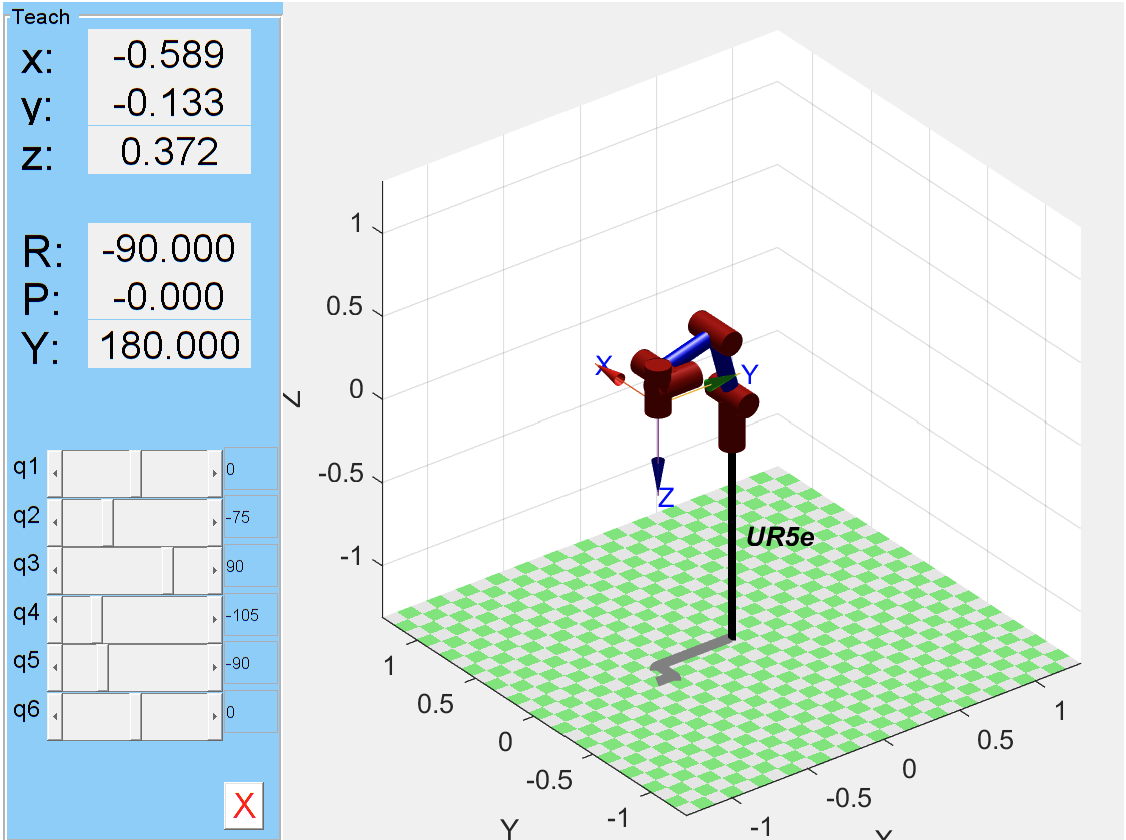
\includegraphics[totalheight=8cm]{Part B Matlab tool result.png}
    \caption{UR5e robot modelled in Matlab at the home position}
    \label{fig:UR5e robot modelled in Matlab}
\end{figure}
\subsubsection{Forward Kinematic Conversion to Attain Pose with Angles in RPY}
By replacing the last code line with fkine(robot, jointConfiguration), we obtain the following matrix result,
\begin{equation*}
    \begin{bmatrix}
        0 & 1 & 0  & -0.5885 \\
        1 & 0 & 0  & -0.1333 \\
        0 & 0 & -1 & 0.3719  \\
        0 & 0 & 0  & 1
    \end{bmatrix}
\end{equation*}
\begin{figure}[H]
    \centering
    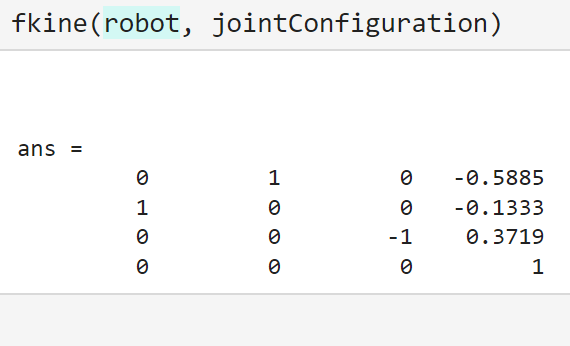
\includegraphics[totalheight=4cm]{Part B Fkine result.png}
    \caption{Matlab fkine result}
    \label{fig:fkine result}
\end{figure}
The only difference between the Matlab result with the manually calculated result in section 2.1 is the final column's values being 1000 times smaller due to using meters instead of millimeters.
\\ \\Once again, to get the pose, we realise that the matrix takes the form of:
\begin{equation*}
    \begin{bmatrix}
        {\begin{array}{ccc|c}&&&\\&R&&T\\&&&\\\hline 0&0&0&1\end{array}}
    \end{bmatrix}
\end{equation*}
So our final joint positions in meters are,
\begin{equation*}
    [-0.5885, -0.1333, 0.3719]
\end{equation*}
And our roll, pitch and yaw values in radians respectively are can be calculated using Matlab's tr2rpy function,
\begin{center}
    \begin{lstlisting}
    rpy = tr2rpy(R);
    % rpy = [3.1416, 0, 1.5708]
    \end{lstlisting}
\end{center}
And thus, our final pose will be,
\begin{equation*}
    [-0.5885, -0.1333, 0.3719, 3.1416, 0, 1.5708]
\end{equation*}
\\ Which matches our manually calculated results when converted to millimeters.
\subsection{Validation of Calculations}
\subsubsection{Screenshot Showing Pose Including the Rotation in RPY Representation}
The following screenshot shows the pose of the UR5e robot in the virtual simulation with a rotation vector.
\begin{figure}[H]
    \centering
    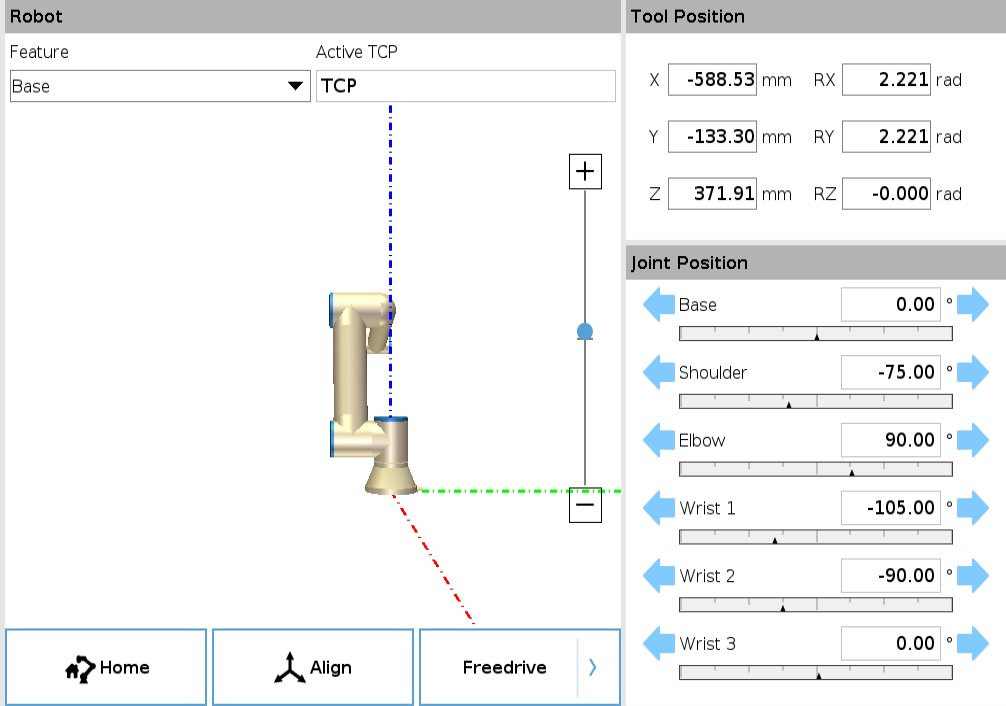
\includegraphics[totalheight=8cm]{Part B Simulation tool result.png}
    \caption{UR5e robot in the home position}
    \label{fig:UR5e robot in the home position}
\end{figure}

When this rotation vector is then converted into RPY, we will get the following angles,
\begin{equation*}
    \begin{bmatrix}
        3.1416 & 0 & 1.5708
    \end{bmatrix}
\end{equation*}
Which validates the calculations performed in previous sections.

